In order to evaluate the training-modified versions of our extrapolation framework, we have to make sure that the evaluation data conforms to the restrictions that we apply to our training set to ensure consistency. In our first trainingmode, we make the restriction on the used $N_\mathrm{max}$ to be lower than 24. In the second training mode, we only use interactions which are SRG evolved using a flow parameter of at least \srg{0.04}. Our evaluation set, consisting of $N_\mathrm{max}$ values up to 12 and of interactions evolved using a flow parameter of \srg{0.04} and \srg{0.08}, already satisfies these requirement.
\begin{figure}[H]
  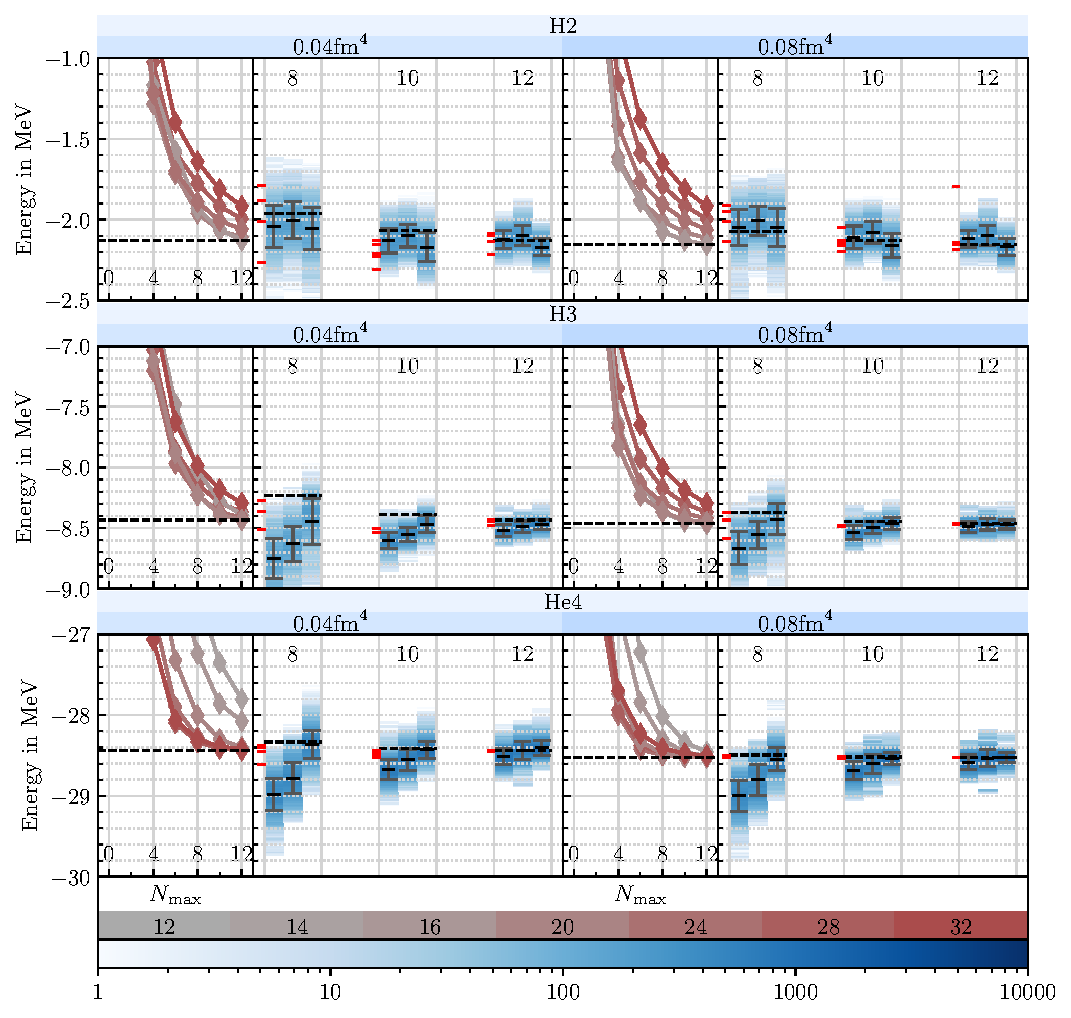
\includegraphics[width=\textwidth]{media/extended_evaluation.pdf}
  \caption{Evaluation of our training modes on the nuclei of \n{2}{H}, \n{3}{H} and \n{4}{He}, using a semi-local momentum space regulated interaction of chiral order 2 with two body interactions and a cutoff at \SI{450}{\mega\electronvolt}. The shown training modes are, in order from left to right, the basic training mode for comparison, the $N_\mathrm{max}$-limitation training mode and the SRG-filter training mode. For each nucleus and each flow parameter, the NCSM sequences are shown on the left and the extrapolations for a given maximum $N_\mathrm{max}$ on the right. For each maximum $N_\mathrm{max}$, the variational boundary is shown as a dotted line, and the classical extrapolations are shown as red ticks.}
  \label{fig:eval_extended}
\end{figure}

In \autoref{fig:eval_extended}, the evaluation of our three nuclei are shown. Each histogram at every $N_\mathrm{max}$ is now divided into three seperate histogram, showcasing the evaluation result for the different training modes. In each stack of histograms, the leftmost is the basic training mode already introduced in \autoref{chap:framework} and assessed in \autoref{chap:reproduction}. The middle histogram corresponds to our first training mode, which restricts the $N_\mathrm{max}$ in the training process to at most 24. The rightmost histogram is our second introduced training mode, which restricts the type of training interactions to SRG evolved interactions with a flow parameter of at least \srg{0.04}.

We again begin by looking at the nuclei \n{3}{H} and \n{4}{He}. For both training modes, we see that the predictions get closer to the variational boundary, which means that the training modes yield overall better predictions, since the sequences are already converged enough. Interestingly, the two trainingmodes seem to only impact the accuracy of the prediction. The uncertainty of both trainingmodes are comparable to the uncertainty of the prediction by the basic extrapolation framework.

If we compare the two trainingmodes for those nuclei, we see that the $N_\mathrm{max}$-limitation mode is less impactful than the SRG-filter mode. This can be explained by the fact that the some of the sequences of the \n{3}{H} and the \n{4}{He} nucleus are already converged enough. Since we explicitly remove bare Hamiltonians in the SRG-filter mode, the training set gets limited to a smaller size of faster-to-converge sequences, thus training the net better to those cases. This can especially be seen in the \n{4}{He} nucleus, where there are sequences which have a
% 3h, 4he:
% in comparison to vanilla: all better
% comparable precision, different accuracy.
% nmax: a bit better
% srg: way better

% 2h:
% nmax worse than vanilla (WHY?)
% nmax geq 10: srg under varbound!

% difference srg
% same as vanilla: extrapolations go up

% srg can handle converged and unconverged sequences
